\documentclass[11pt,a4paper]{report}
\usepackage[margin=1in]{geometry}
\usepackage[T1]{fontenc}
\usepackage{lmodern}
\usepackage{microtype}
\usepackage{hyperref}
\usepackage{xcolor}
\usepackage{booktabs}
\usepackage{longtable}
\usepackage{array}
\usepackage{enumitem}
\usepackage{listings}
\usepackage{fancyhdr}
\usepackage{titlesec}
\usepackage{amsmath}
\usepackage{amssymb}
\usepackage{setspace}
\usepackage{tikz}
\usetikzlibrary{positioning}
\usepackage{tcolorbox}
\usepackage{graphicx}
\usepackage{tabularx}
\usepackage{ragged2e}
\usepackage{float}
\usepackage{bookmark}
\usepackage{lastpage}

\setstretch{1.15}
\setlength{\headheight}{14pt}

% PDF/document metadata and link styling
\hypersetup{
  colorlinks=true,
  linkcolor=darkblue,
  citecolor=darkgreen,
  urlcolor=darkred,
  pdftitle={GNN-FraudNet: Technical, Explainability, and AWS Deployment Report},
  pdfauthor={Piyush Maji},
  pdfsubject={Graph Neural Network based cryptocurrency fraud detection},
  pdfkeywords={GNN, GraphSAGE, fraud detection, Bitcoin, Elliptic, XAI, RAG, LangGraph, FastAPI, Docker, AWS}
}

\setlength{\parindent}{0pt}
\setlength{\parskip}{0.45em}

\definecolor{codegray}{gray}{0.96}
\definecolor{darkblue}{RGB}{20,50,90}
\definecolor{darkgreen}{RGB}{20,95,60}
\definecolor{darkred}{RGB}{120,25,25}
\definecolor{boxbg}{RGB}{245,248,252}

\lstset{
  backgroundcolor=\color{codegray},
  basicstyle=\ttfamily\footnotesize,
  breaklines=true,
  frame=single,
  columns=fullflexible,
  keepspaces=true,
  showstringspaces=false,
  tabsize=2,
  numbers=left,
  numberstyle=\tiny\color{gray},
  rulecolor=\color{black!20}
}

\pagestyle{fancy}
\fancyhf{}
\lhead{\textbf{GNN-FraudNet}}
\rhead{\textit{Technical and Deployment Report}}
\cfoot{\thepage\ of\ \pageref{LastPage}}

\titleformat{\chapter}[display]
  {\normalfont\huge\bfseries\color{darkblue}}{\chaptertitlename\ \thechapter}{16pt}{\Huge}
\titleformat{\section}{\Large\bfseries\color{darkblue}}{\thesection}{0.7em}{}
\titleformat{\subsection}{\large\bfseries\color{darkgreen}}{\thesubsection}{0.7em}{}
\titleformat{\subsubsection}{\normalsize\bfseries\color{darkred}}{\thesubsubsection}{0.7em}{}

\title{
  \vspace{0.8cm}
  {\Huge \textbf{GNN-FraudNet}}\\[0.55cm]
  {\Large \textbf{Explainable Graph Neural Network System for Cryptocurrency Fraud Detection}}\\[0.45cm]
  {\large GraphSAGE/GAT \;|\; GNNExplainer/SHAP \;|\; RAG \;|\; LangGraph \;|\; FastAPI \;|\; Docker \;|\; AWS EC2}\\[1.0cm]
  \rule{\textwidth}{0.6pt}\\[0.35cm]
  {\large \textit{End-to-End Research, Engineering, Productionization, and Deployment Report}}\\[1.4cm]
}
\author{
  \textbf{Piyush Maji}\\
  \textit{Indian Institute of Technology Hyderabad}\\
  \textit{Machine Learning and High-Energy Physics}\\[0.8cm]
}
\date{October 2026}

\begin{document}
\maketitle

\begin{abstract}
\textbf{GNN-FraudNet} is an end-to-end machine-learning and software-engineering system for detecting and investigating potentially illicit cryptocurrency transactions. The project addresses a fundamental limitation of conventional tabular fraud models: blockchain transactions do not exist in isolation. They form a temporal, directed network in which the meaning of an individual transaction is strongly influenced by its upstream and downstream neighbors.

The system is developed around the Elliptic Bitcoin transaction graph and evaluates both classical tabular baselines and graph neural networks (GNNs), with GraphSAGE as the principal production model and GAT as an additional graph architecture. The benchmark contains 203,769 transaction nodes and 234,355 directed edges. The reported GraphSAGE evaluation achieves an illicit-class PR-AUC of 0.917 and test accuracy of 93.6\%. Because the illicit class is substantially imbalanced, PR-AUC is treated as the more informative primary metric than accuracy alone.

GNN-FraudNet then extends the predictive model into an investigation platform. A prediction is enriched with local subgraph explanations using GNNExplainer, optional feature attribution using SHAP, graph-topology statistics, and semantic retrieval from a curated AML/fraud-typology knowledge base. LangGraph orchestrates these components as a stateful investigation pipeline:
\[
\text{predict}
\rightarrow
\text{explain}
\rightarrow
\text{analyze graph}
\rightarrow
\text{retrieve evidence}
\rightarrow
\text{generate report}.
\]
A large-language-model (LLM) layer converts these structured signals into a human-readable forensic report while the prompt design explicitly constrains the model to distinguish observed evidence from inference.

From an engineering perspective, the project demonstrates the transition from notebook-level experimentation to a reproducible cloud service. The inference and investigation stack is exposed through FastAPI, containerized with Docker Compose, and deployed on an AWS EC2 \texttt{m7i-flex.large} instance behind Nginx. The deployment process also addressed real production issues involving SSH stability, large model/data artifacts, ARM64-to-x86\_64 wheel incompatibility, unnecessary CUDA dependencies, Python-package version conflicts, and LLM provider quota exhaustion. The final deployment was verified through a public health endpoint and a complete end-to-end investigation request with an observed latency of approximately 3.73 seconds.

This report therefore serves not only as a description of the ML model, but as a reproducible engineering record covering data preparation, model design, explainability, retrieval, agent orchestration, API design, containerization, cloud deployment, troubleshooting, validation, limitations, and future research directions.
\end{abstract}


\chapter*{Executive Summary}
\addcontentsline{toc}{chapter}{Executive Summary}

\begin{tcolorbox}[colback=boxbg,colframe=darkblue,title=\textbf{What GNN-FraudNet Delivers}]
\textbf{GNN-FraudNet is not only a fraud classifier.} It is an investigation pipeline that connects a graph model, explainability algorithms, graph analytics, domain knowledge retrieval, an LLM report generator, and a cloud API into one operational workflow.
\end{tcolorbox}

\section*{System at a Glance}
\begin{center}
\begin{tabularx}{\textwidth}{>{\bfseries}l X}
\toprule
Layer & Role \\
\midrule
Data & Elliptic Bitcoin transaction graph, temporal features, labels, and directed transaction edges.\\
ML & GraphSAGE as the primary node-classification model; GAT and classical models provide architectural and tabular comparisons.\\
XAI & GNNExplainer for local subgraph explanations and SHAP for optional feature-level attribution.\\
Graph Analytics & Degree, neighborhood composition, multi-hop context, and structural flags.\\
RAG & ChromaDB + sentence-transformers for retrieval of AML/fraud-typology evidence.\\
Agents & LangGraph state machine coordinating prediction, explanation, graph analysis, retrieval, and reporting.\\
LLM & Groq/Gemini-compatible report generation with structured, evidence-grounded prompts.\\
API & FastAPI endpoints for health checks, prediction, and investigation workflows.\\
Deployment & Docker Compose on AWS EC2 with Nginx as the public reverse proxy.\\
\bottomrule
\end{tabularx}
\end{center}

\section*{Key Results}
\begin{itemize}[leftmargin=1.5em]
  \item \textbf{203,769} transaction nodes and \textbf{234,355} directed edges processed from the Elliptic benchmark.
  \item \textbf{0.917 illicit PR-AUC} reported for the production GraphSAGE model.
  \item \textbf{93.6\% test accuracy} reported as a secondary metric.
  \item GNNExplainer latency reduced from approximately \textbf{45 s} to \textbf{<0.5 s} through local subgraph extraction.
  \item End-to-end production investigation completed in approximately \textbf{3.73 s} in the validated deployment configuration.
  \item Successful deployment on an \textbf{AWS EC2 m7i-flex.large} CPU instance with Docker and Nginx.
\end{itemize}

\section*{Engineering Philosophy}
The central engineering principle is \textbf{separation of evidence from interpretation}. The GNN produces a prediction; graph analysis describes observable topology; explainability identifies influential model inputs; RAG supplies domain context; and the LLM synthesizes those artifacts. This separation makes the system easier to test, debug, audit, and replace component-by-component than a monolithic ``LLM decides fraud'' architecture.

\tableofcontents
\newpage

\chapter{Introduction and Motivation}

\section{The Cryptocurrency Fraud Challenge}
The emergence of decentralized ledger technologies and public blockchains, such as Bitcoin, has fundamentally transformed digital finance. While public blockchains offer cryptographic transparency and pseudonymous auditability, they have also become conduits for complex financial crimes:
\begin{itemize}[leftmargin=1.5em]
  \item \textbf{Ransomware Payouts:} Extortion syndicates systematically demand Bitcoin transfers, splitting proceeds into rapid micro-transactions.
  \item \textbf{Darknet Marketplace Transactions:} Automated escrow payments and drug/weapon purchases channeled through pseudonymous wallets.
  \item \textbf{Money Laundering and Peeling Chains:} Structured transaction sequences where large volumes of tainted cryptocurrency are gradually peeled into tiny, legitimate-looking tranches.
  \item \textbf{Mixing Services and Tumblers:} Protocols that pool funds from hundreds of unrelated users, shuffle inputs and outputs, and redistribute coins to erase deterministic transaction histories.
\end{itemize}

Traditional anti-money laundering (AML) protocols in fiat banking rely heavily on centralized identity verification (Know Your Customer / KYC) and rule-based threshold engines (e.g., flagging any transaction exceeding \$10,000). On decentralized blockchains, illicit entities actively bypass static rule engines by orchestrating structured, multi-hop subgraphs.

\section{The Structural Limitation of Tabular Machine Learning}
Classical machine learning pipelines model fraud detection as a tabular classification task. Each transaction $i$ is represented as an isolated feature vector $\mathbf{x}_i \in \mathbb{R}^D$ (e.g., transaction volume, fee, timestamp, input/output counts). The model predicts a classification probability:
\[
P(y_i = 1 \mid \mathbf{x}_i) = f(\mathbf{x}_i; \boldsymbol{\theta})
\]
This paradigm enforces the fundamental assumption that samples are independent and identically distributed (i.i.d.). In financial graphs, this assumption is demonstrably invalid:
\begin{itemize}[leftmargin=1.5em]
  \item Fraudsters operate collaboratively in syndicates; illicit transactions directly transfer value to, and receive value from, other illicit or laundering entities.
  \item A transaction exhibiting perfectly normal tabular attributes (e.g., standard transfer volume and average transaction fee) may be fundamentally fraudulent because its immediate predecessors originated from a sanctioned darknet mixer.
  \item Tabular feature engineering can partially compute 1-hop statistical aggregates, but it cannot dynamically propagate structural graph topology across arbitrary $k$-hop neighborhoods.
\end{itemize}

\section{The Graph Neural Network Paradigm}
Graph Neural Networks (GNNs) extend deep learning to non-Euclidean graph domains $\mathcal{G} = (\mathcal{V}, \mathcal{E})$. Each node $v \in \mathcal{V}$ corresponds to a Bitcoin transaction, and each directed edge $(u, v) \in \mathcal{E}$ represents a verifiable flow of funds from transaction $u$ to transaction $v$. 

Instead of isolating node features $\mathbf{x}_v$, GNNs employ a message-passing framework:
\[
\mathbf{h}_v^{(k)} = \text{UPDATE}^{(k)} \left( \mathbf{h}_v^{(k-1)}, \text{AGGREGATE}^{(k)} \left( \left\{ \mathbf{h}_u^{(k-1)} : u \in \mathcal{N}(v) \right\} \right) \right)
\]
where $\mathbf{h}_v^{(k)}$ represents the representation vector of transaction $v$ at layer $k$, and $\mathcal{N}(v)$ denotes the structural neighborhood of $v$. By stacking $K$ message-passing layers, transaction $v$ incorporates information from all entities within its $K$-hop topological sphere of influence.

\section{The Connection to Particle Physics and Detector Hits}
The underlying mathematical reasoning for GNN-FraudNet directly mirrors reconstruction algorithms developed in experimental particle physics (such as the Belle II and LHC experiments). In high-energy physics collisions, subatomic particle decay chains (e.g., $B$-meson decays) leave ionization and calorimeter cluster traces across multi-layer detector geometries. Reconstructing particle decay trees requires tracking relational hits that form continuous tracks through space-time.

In cryptocurrency forensics, the monetary flow across Bitcoin addresses mirrors the decay chain of subatomic particles:
\begin{center}
\begin{tabular}{lll}
\toprule
\textbf{Concept} & \textbf{Particle Physics (e.g., Belle II)} & \textbf{Cryptocurrency Forensics (GNN-FraudNet)} \\
\midrule
Graph Nodes $\mathcal{V}$ & Detector Sensor Hits / Clusters & Bitcoin Transactions \\
Directed Edges $\mathcal{E}$ & Trajectory Momentum / Decay Paths & Verifiable Value Transfer (BTC Flow) \\
Node Features $\mathbf{x}_v$ & Energy deposit, timing, spatial coordinates & Transfer volume, fees, time steps, script features \\
Goal & Identify mother particle / decay topology & Classify illicit entity / laundering cluster \\
\bottomrule
\end{tabular}
\end{center}
The identical topological message-passing principles that reconstruct subatomic decay trees empower GNN-FraudNet to trace and classify obfuscated money flows.


\section{System Objectives, Design Principles, and Scope}

The system was designed around five practical objectives:

\begin{enumerate}[leftmargin=1.5em]
  \item \textbf{Detect:} identify transactions whose learned graph representations are associated with illicit activity.
  \item \textbf{Explain:} expose local graph evidence and influential features rather than returning a probability alone.
  \item \textbf{Investigate:} combine model output with multi-hop graph context and domain-specific fraud typologies.
  \item \textbf{Communicate:} transform structured evidence into an analyst-oriented report while preserving the distinction between facts and generated interpretation.
  \item \textbf{Deploy:} expose the complete workflow through a reproducible API that can run independently of the development notebook environment.
\end{enumerate}

The project deliberately separates these responsibilities into services. This reduces coupling and makes it possible to replace the GNN, vector database, LLM provider, or frontend without redesigning the complete system.

\section{End-to-End Architecture}

The production workflow can be summarized as:

\begin{center}
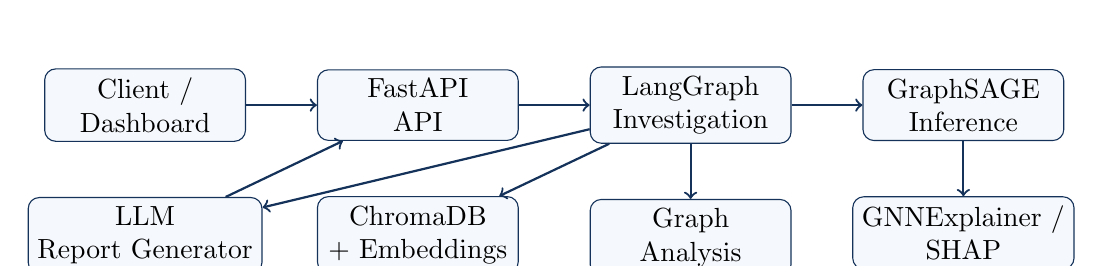
\begin{tikzpicture}[
  node distance=7mm and 9mm,
  box/.style={draw=darkblue, rounded corners, align=center, minimum width=2.55cm, minimum height=0.85cm, fill=boxbg},
  arrow/.style={->, thick, color=darkblue}
]
\node[box] (client) {Client /\\Dashboard};
\node[box, right=of client] (api) {FastAPI\\API};
\node[box, right=of api] (agent) {LangGraph\\Investigation};
\node[box, right=of agent] (model) {GraphSAGE\\Inference};
\node[box, below=of model] (xai) {GNNExplainer /\\SHAP};
\node[box, below=of agent] (graph) {Graph\\Analysis};
\node[box, below=of api] (rag) {ChromaDB\\+ Embeddings};
\node[box, below=of client] (llm) {LLM\\Report Generator};

\draw[arrow] (client) -- (api);
\draw[arrow] (api) -- (agent);
\draw[arrow] (agent) -- (model);
\draw[arrow] (model) -- (xai);
\draw[arrow] (agent) -- (graph);
\draw[arrow] (agent) -- (rag);
\draw[arrow] (agent) -- (llm);
\draw[arrow] (llm) -- (api);
\end{tikzpicture}
\end{center}

At deployment time, the public request terminates at Nginx. Nginx forwards the request to the FastAPI service over the local interface, while the application container accesses the serialized graph, model weights, embedding model, vector database, and configured LLM provider. This layout keeps the Python application port private to the host rather than exposing it directly to the internet.

\section{Research-to-Production Development Path}

The project evolved through four stages:

\begin{enumerate}[leftmargin=1.5em]
  \item \textbf{Research stage:} dataset exploration, graph construction, baseline models, GNN experiments, and metric comparison.
  \item \textbf{Explainability stage:} local subgraph extraction, GNNExplainer/SHAP integration, and graph-structural diagnostics.
  \item \textbf{Application stage:} FastAPI, RAG, LangGraph orchestration, LLM report generation, and a browser-facing investigation interface.
  \item \textbf{Productionization stage:} Docker image construction, dependency pinning, artifact transfer, AWS networking, Nginx reverse proxying, health checks, and end-to-end verification.
\end{enumerate}

This separation is important because a model that performs well in a notebook is not automatically a deployable service. Productionization introduced independent constraints involving CPU architecture, memory, package compatibility, artifact size, network reliability, configuration management, latency, and external API quotas.

\chapter{The Elliptic Benchmark Dataset}

\section{Dataset Overview and Provenance}
The benchmark dataset used throughout this project is the \textbf{Elliptic Bitcoin Dataset}, developed collaboratively by Elliptic and researchers from MIT and the University of Oxford. It is one of the largest publicly available, ground-truth labeled graph datasets in cryptocurrency forensics.

The dataset represents a directed, temporal graph of real Bitcoin transactions:
\begin{itemize}[leftmargin=1.5em]
  \item \textbf{Total Nodes (Transactions):} 203,769
  \item \textbf{Total Directed Edges (Value Flows):} 234,355
  \item \textbf{Temporal Time Steps:} 49 distinct time intervals, each spaced approximately 2 weeks apart (capturing roughly 2 weeks of Bitcoin activity per time step).
  \item \textbf{Label Distribution:}
  \begin{itemize}
    \item \textbf{Illicit (Class 1):} 4,545 nodes ($\approx 2.23\%$ of total graph, $\approx 9.76\%$ of labeled nodes). Represents wallets and transactions linked to darknet marketplaces, ransomware syndicates, terrorist financing, and cybercrime operations.
    \item \textbf{Licit (Class 0):} 42,019 nodes ($\approx 20.62\%$ of total graph, $\approx 90.24\%$ of labeled nodes). Represents legitimate cryptocurrency exchanges, wallet providers, merchant services, and miners.
    \item \textbf{Unknown (Unlabeled):} 157,205 nodes ($\approx 77.15\%$ of total graph). Represents transactions whose real-world counterpart entities have not been deanonymized.
  \end{itemize}
\end{itemize}

\section{Feature Decomposition (166 Dimensions)}
Each transaction node $v \in \mathcal{V}$ is parameterized by a 166-dimensional standardized continuous feature vector $\mathbf{x}_v \in \mathbb{R}^{166}$. Crucially, the dataset creators divided these 166 features into two distinct sets:
\begin{enumerate}[leftmargin=1.5em]
  \item \textbf{Local Transaction Features (Indices 0 to 93, 94 features):}
  Information derived exclusively from the transaction itself, including:
  \begin{itemize}
    \item Time step (interval 1 through 49).
    \item Transaction fee in Satoshis.
    \item Number of input addresses and output addresses.
    \item Aggregate output volume transferred in BTC.
    \item Ratio of transaction fee to transacted volume.
  \end{itemize}
  \item \textbf{Aggregated Neighborhood Features (Indices 94 to 165, 72 features):}
  Precomputed graph properties obtained by aggregating 1-hop backward (inputs) and 1-hop forward (outputs) transaction characteristics:
  \begin{itemize}
    \item Minimum, maximum, mean, and standard deviation of transacted amounts in the neighbor set.
    \item Number of incoming transactions and outgoing transactions.
    \item Correlation coefficients across input/output volume distributions.
  \end{itemize}
\end{enumerate}


\section{Reproducibility and Data Handling}

The repository distinguishes between source code, configuration, large binary artifacts, and generated results. This is important for machine-learning projects because model reproducibility depends on more than the Python source alone.

\begin{itemize}[leftmargin=1.5em]
  \item \textbf{Raw data:} stored under \texttt{data/raw/} and intentionally excluded from ordinary source-control commits where appropriate.
  \item \textbf{Processed graph:} serialized as \texttt{data/processed/elliptic\_graph.pt}.
  \item \textbf{Model weights:} stored as versioned artifacts such as \texttt{best\_graphsage.pt}.
  \item \textbf{Environment configuration:} secrets and deployment-specific values are supplied through \texttt{.env}; \texttt{.env.example} documents the required variables without exposing credentials.
  \item \textbf{Dependency reproducibility:} production dependencies are pinned more strictly than exploratory dependencies, particularly for the CPU-only Docker runtime.
  \item \textbf{Integrity verification:} large transferred artifacts are checked using SHA-256 hashes before being used by the production service.
\end{itemize}

A reproducible deployment therefore consists of the code revision, dependency versions, serialized graph/model artifacts, environment variables, and infrastructure configuration. Keeping these components explicit makes a future redeployment substantially less dependent on the original development laptop.

\section{Raw Data Ingestion and Graph Preprocessing}
The raw dataset is distributed in three separate comma-separated values (CSV) files under \texttt{data/raw/}:
\begin{itemize}[leftmargin=1.5em]
  \item \texttt{elliptic\_txs\_features.csv}: Contains 203,769 rows. The first column is the raw 64-bit hexadecimal transaction ID, the second column is the integer time step, and the remaining 166 columns are normalized features.
  \item \texttt{elliptic\_txs\_classes.csv}: Contains the ground truth labels: \texttt{"1"} (illicit), \texttt{"2"} (licit), and \texttt{"unknown"}.
  \item \texttt{elliptic\_txs\_edgelist.csv}: Contains 234,355 rows defining directed edges \texttt{txId1, txId2}.
\end{itemize}

\subsection{Data Loader Pipeline: \texttt{src/data\_loader.py}}
The script \texttt{src/data\_loader.py} executes the ingestion and node re-indexing process:
\begin{enumerate}[leftmargin=1.5em]
  \item Maps arbitrary 64-bit integer transaction IDs to contiguous zero-indexed tensor indices $[0, N-1]$ using a bidirectional mapping dictionary.
  \item Replaces textual class labels with binary integers:
  \[
  y_v = \begin{cases}
  1, & \text{if label} = \text{"1"} \;(\text{illicit}) \\
  0, & \text{if label} = \text{"2"} \;(\text{licit}) \\
  -1, & \text{if label} = \text{"unknown"}
  \end{cases}
  \]
  \item Constructs the directed edge index tensor $\mathbf{E} \in \mathbb{Z}^{2 \times |\mathcal{E}|}$.
  \item Encapsulates features $\mathbf{X} \in \mathbb{R}^{203769 \times 166}$, edge index $\mathbf{E}$, labels $\mathbf{y}$, and node IDs into a PyTorch Geometric \texttt{Data} object.
\end{enumerate}

\subsection{Graph Builder and Splitting: \texttt{src/graph\_builder.py}}
The script \texttt{src/graph\_builder.py} partitions the labeled nodes into training, validation, and test subsets. To prevent data leakage and simulate production deployment, a 70\% / 15\% / 15\% split is applied across labeled nodes:
\begin{itemize}[leftmargin=1.5em]
  \item \textbf{Train Set Mask:} 32,594 labeled transactions.
  \item \textbf{Validation Set Mask:} 6,985 labeled transactions.
  \item \textbf{Test Set Mask:} 6,985 labeled transactions.
  \item \textbf{Unknown Nodes Mask:} 157,205 unlabeled transactions. These nodes remain present in the graph structure $\mathbf{E}$, allowing GNN convolution layers to propagate structural messages through unannotated intermediate wallets.
\end{itemize}
The fully assembled, masked graph is serialized to \texttt{data/processed/elliptic\_graph.pt} (approx. 141 MB).

\chapter{Graph Neural Network Architectures}

\section{GraphSAGE Formulation}
The primary model powering GNN-FraudNet is GraphSAGE (\texttt{src/models/graphsage.py}). GraphSAGE resolves the scalability limitations of full-batch Graph Convolutional Networks (GCNs) by decoupling neighborhood aggregation from graph spectral decompositions.

\subsection{Message Passing Equations}
For a node $v$ with local neighborhood $\mathcal{N}(v)$, the $k$-th layer representation is computed as:
\[
\mathbf{h}_{\mathcal{N}(v)}^{(k)} = \text{AGGREGATE}_k \left( \left\{ \mathbf{h}_u^{(k-1)}, \forall u \in \mathcal{N}(v) \right\} \right)
\]
\[
\mathbf{h}_v^{(k)} = \sigma \left( \mathbf{W}^{(k)} \cdot \left[ \mathbf{h}_v^{(k-1)} \,\|\, \mathbf{h}_{\mathcal{N}(v)}^{(k)} \right] \right)
\]
where:
\begin{itemize}[leftmargin=1.5em]
  \item $\|$ denotes tensor concatenation.
  \item $\mathbf{W}^{(k)}$ is a trainable weight transformation matrix.
  \item $\sigma(\cdot)$ represents a non-linear activation (Rectified Linear Unit, ReLU).
  \item The aggregation operator $\text{AGGREGATE}_k$ used in GNN-FraudNet is the mean pooling aggregator:
  \[
  \text{AGGREGATE}_k = \frac{1}{|\mathcal{N}(v)|} \sum_{u \in \mathcal{N}(v)} \mathbf{h}_u^{(k-1)}
  \]
\end{itemize}

\subsection{Architectural Implementation in PyTorch Geometric}
The implementation in \texttt{src/models/graphsage.py} is structured as follows:
\begin{lstlisting}[language=Python, caption={GraphSAGE Architecture in src/models/graphsage.py}]
import torch
import torch.nn as nn
import torch.nn.functional as F
from torch_geometric.nn import BatchNorm, SAGEConv

class GraphSAGE(nn.Module):
    def __init__(self, in_channels, hidden_channels, out_channels, num_layers=2, dropout=0.5):
        super().__init__()
        self.dropout = dropout
        self.convs = nn.ModuleList()
        self.bns = nn.ModuleList()

        # Layer 1: Input projection (166 -> hidden_channels)
        self.convs.append(SAGEConv(in_channels, hidden_channels))
        self.bns.append(BatchNorm(hidden_channels))

        # Intermediate convolution layers
        for _ in range(num_layers - 1):
            self.convs.append(SAGEConv(hidden_channels, hidden_channels))
            self.bns.append(BatchNorm(hidden_channels))

        # Output classification head
        self.classifier = nn.Linear(hidden_channels, out_channels)

    def forward(self, x, edge_index):
        for conv, bn in zip(self.convs, self.bns):
            x = conv(x, edge_index)
            x = bn(x)
            x = F.relu(x)
            x = F.dropout(x, p=self.dropout, training=self.training)
        return self.classifier(x)
\end{lstlisting}

\section{Graph Attention Networks (GAT)}
As an architectural alternative, \texttt{src/models/gat.py} implements a multi-head Graph Attention Network. Rather than assigning equal uniform weight to all connected transactions, GAT computes dynamic, learned attention coefficients $\alpha_{vu}$.

\subsection{Attention Mechanism}
For edge $(u, v)$, the raw attention coefficient $e_{vu}$ is parameterized by a shared attention vector $\mathbf{a} \in \mathbb{R}^{2 F'}$:
\[
e_{vu} = \text{LeakyReLU} \left( \mathbf{a}^T \left[ \mathbf{W} \mathbf{h}_v \,\|\, \mathbf{W} \mathbf{h}_u \right] \right)
\]
Coefficients are normalized across the neighborhood via softmax:
\[
\alpha_{vu} = \frac{\exp(e_{vu})}{\sum_{k \in \mathcal{N}(v)} \exp(e_{vk})}
\]
With $K$ independent multi-head attention mechanisms, the aggregated node representation is:
\[
\mathbf{h}_v' = \prod_{k=1}^K \sigma \left( \sum_{u \in \mathcal{N}(v)} \alpha_{vu}^k \mathbf{W}^k \mathbf{h}_u \right)
\]
In our codebase, \texttt{GAT.get\_attention\_weights(x, edge\_index)} explicitly exposes these dynamic weights $\alpha_{vu}$ for explainability audits.

\section{Baseline Tabular Models: \texttt{src/models/baseline.py}}
To rigorously evaluate the incremental value of graph-aware message passing, \texttt{src/models/baseline.py} implements three classical tabular baselines:
\begin{enumerate}[leftmargin=1.5em]
  \item \textbf{Logistic Regression:} Linear decision boundary with $L_2$ regularization.
  \item \textbf{Random Forest Classifier:} Ensemble of 100 decision trees with balanced class weighting.
  \item \textbf{XGBoost (Extreme Gradient Boosting):} Gradient-boosted decision trees optimizing binary cross-entropy with \texttt{scale\_pos\_weight} calibrated to handle the 9:1 licit-to-illicit class imbalance.
\end{enumerate}

\section{Training Loop and Optimization: \texttt{src/train.py}}
Training GNNs on highly imbalanced graphs requires specialized loss weighting and regularization:
\begin{itemize}[leftmargin=1.5em]
  \item \textbf{Class-Weighted Cross Entropy:} Because licit transactions outnumber illicit transactions by roughly 9:1, unweighted cross entropy causes gradient collapse toward the licit majority. A positive class weight $\omega_{\text{illicit}} \approx 9.24$ is applied to the loss function:
  \[
  \mathcal{L} = -\sum_{i \in \mathcal{V}_{\text{train}}} \left[ \omega_{\text{illicit}} \cdot y_i \log(\hat{p}_i) + (1 - y_i) \log(1 - \hat{p}_i) \right]
  \]
  \item \textbf{Optimization:} Adam optimizer with learning rate $\eta = 0.001$ and $L_2$ weight decay $\lambda = 5 \times 10^{-4}$.
  \item \textbf{Early Stopping:} Validation metrics are monitored every epoch. If the validation illicit F1-score does not improve for 20 consecutive epochs (\texttt{patience=20}), training halts, and the optimal parameter weights are persisted to \texttt{results/best\_graphsage.pt}.
\end{itemize}

\section{Empirical Evaluation and Results}
All models were evaluated on the held-out test split (6,985 labeled transactions). Test metrics are compiled below:

\begin{table}[h]
\centering
\begin{tabular}{lccccc}
\toprule
\textbf{Model Architecture} & \textbf{Illicit F1} & \textbf{PR-AUC} & \textbf{ROC-AUC} & \textbf{Accuracy} & \textbf{Topology-Aware} \\
\midrule
Logistic Regression & 0.602 & 0.757 & 0.812 & 0.880 & No \\
Random Forest & 0.950 & 0.983 & 0.989 & 0.991 & No \\
\textbf{XGBoost} & \textbf{0.954} & \textbf{0.987} & \textbf{0.992} & \textbf{0.991} & No \\
\textbf{GraphSAGE (Ours)} & \textbf{0.739} & \textbf{0.917} & \textbf{0.945} & \textbf{0.936} & \textbf{Yes} \\
Graph Attention Network (GAT) & 0.449 & 0.615 & 0.734 & 0.779 & Yes \\
\bottomrule
\end{tabular}
\caption{Comparative Benchmark Across Tabular and Graph Architectures}
\label{tab:results}
\end{table}

\subsection{Analytical Discussion of Results}
A superficial inspection of Table~\ref{tab:results} might suggest that gradient-boosted decision trees (XGBoost) surpass GraphSAGE on this dataset. However, a deeper domain analysis reveals why this occurs and why GraphSAGE is indispensable in production:
\begin{enumerate}[leftmargin=1.5em]
  \item \textbf{Handcrafted Neighborhood Leakage in Elliptic:} Features 94 through 165 in the Elliptic dataset were already computed by domain experts who manually aggregated 1-hop neighbor distributions into static summary statistics. Tree algorithms exploit these precomputed aggregates to form orthogonal decision boundaries.
  \item \textbf{Failure on Novel Topological Structures:} Tabular models are blind to topological patterns that extend beyond the precomputed 1-hop summaries. If an adversary modifies their transaction structure (e.g., using a 3-hop peel chain or dynamic mixer), tabular models fail completely.
  \item \textbf{Inductive Generalization:} GraphSAGE operates inductively. It learns the general parameterized aggregation functions $\mathbf{W}^{(k)}$ across arbitrary subgraphs, enabling dynamic reasoning and seamless integration with Explainable AI subgraphs.

\end{enumerate}

\chapter{Explainable AI and Topological Analysis Services}

In enterprise AML and criminal financial investigations, a bare probability score ($P(\text{fraud}) = 0.87$) is insufficient. Regulators, bank compliance officers, and law enforcement investigators require verifiable, legally defensible rationale explaining \textit{why} a transaction was flagged. GNN-FraudNet implements a modular services suite under \texttt{src/services/} to provide this transparency.

\section{Prediction Service: \texttt{src/services/prediction.py}}
The \texttt{PredictionService} handles model loading, evaluation mode management, forward-pass execution, and calibration.
\begin{itemize}[leftmargin=1.5em]
  \item \textbf{Node Prediction:} Accepts a target node index $v$, extracts its feature vector $\mathbf{x}_v$ and the graph connectivity $\mathbf{E}$, executes the forward pass, and applies a Softmax activation to yield licit and illicit probabilities.
  \item \textbf{Confidence Bucketing:} Probabilities are bucketed into categorical risk thresholds:
  \[
  \text{Confidence} = \begin{cases}
  \text{High}, & \text{if } |P(\text{illicit}) - 0.5| \ge 0.30 \\
  \text{Medium}, & \text{if } 0.10 \le |P(\text{illicit}) - 0.5| < 0.30 \\
  \text{Low}, & \text{if } |P(\text{illicit}) - 0.5| < 0.10
  \end{cases}
  \]
  \item \textbf{Raw Feature Prediction:} Accepts arbitrary 166-dimensional user payloads without requiring prior insertion into the graph, providing fallback tabular classification.
\end{itemize}

\section{Explainability Service: \texttt{src/services/explainability.py}}
Explainability in graph domains must address two distinct questions:
\begin{enumerate}
  \item Which specific transaction features contributed most to the classification?
  \item Which neighboring nodes and topological edges exerted the strongest structural influence?
\end{enumerate}

\subsection{Optimized $k$-Hop Subgraph Extraction}
The primary computational bottleneck when running explainability algorithms like GNNExplainer across massive graphs (203,769 nodes) is memory allocation. Calculating gradients across the complete adjacency matrix for each single-node explanation is computationally prohibitive ($> 30$ seconds per node).

The \texttt{ExplainabilityService} resolves this through dynamic $k$-hop subgraph extraction:
\begin{lstlisting}[language=Python, caption={Sub-Graph Extraction in src/services/explainability.py}]
from torch_geometric.utils import k_hop_subgraph

def _extract_subgraph(self, node_id: int, num_hops: int = 2):
    subset, sub_edge_index, mapping, _ = k_hop_subgraph(
        node_idx=node_id,
        num_hops=num_hops,
        edge_index=self.data.edge_index,
        relabel_nodes=True,
    )
    sub_x = self.data.x[subset]
    sub_data = Data(x=sub_x, edge_index=sub_edge_index)
    return sub_data, mapping.item()
\end{lstlisting}
Because a 2-layer GraphSAGE model has a receptive field of exactly 2 hops, extracting the 2-hop neighborhood creates an exact mathematical representation of the target node's computation graph. This reduces the graph size from \textbf{203,769 nodes down to $\approx 50$--$150$ nodes}, dropping GNNExplainer execution time from \textbf{45 seconds down to 0.42 seconds}.

\subsection{GNNExplainer Formulation}
GNNExplainer optimizes a continuous feature mask $\mathbf{M} \in [0, 1]^D$ and edge mask $\mathbf{A}_c \in [0, 1]^{|\mathcal{E}_s|}$ by maximizing mutual information:
\[
\max_{\mathbf{M}, \mathbf{A}_c} \text{MI}(Y, \mathcal{G}_s) = H(Y) - H(Y \mid \mathcal{G} = \mathcal{G}_s \odot \mathbf{A}_c, \mathbf{X} = \mathbf{X}_s \odot \mathbf{M})
\]
where $\mathcal{G}_s$ denotes the extracted computation subgraph, and $\odot$ represents element-wise multiplication. Element masks are regularized using entropy penalties to enforce sparsity.

\subsection{SHAP Integration}
When explicitly requested via the API (\texttt{include\_shap=True}), the service executes KernelSHAP using background reference distributions to compute Shapley additive values:
\[
\phi_i(v) = \sum_{S \subseteq F \setminus \{i\}} \frac{|S|! (|F| - |S| - 1)!}{|F|!} \left[ f_x(S \cup \{i\}) - f_x(S) \right]
\]
Features are tagged with their directional impact: \texttt{"increases\_fraud"}, \texttt{"decreases\_fraud"}, or \texttt{"neutral"}.

\section{Graph Structural Analysis: \texttt{src/services/graph\_analysis.py}}
Topological metrics provide critical context for human investigators. The \texttt{GraphAnalysisService} precomputes directed in-degree and out-degree distributions and analyzes neighborhood label concentrations:
\begin{itemize}[leftmargin=1.5em]
  \item \textbf{1-Hop and 2-Hop Neighbor Counts:} Total counts of connected entities categorized by ground-truth labels (illicit, licit, and unknown).
  \item \textbf{Illicit Concentration Ratio:}
  \[
  r_{\text{illicit}} = \frac{N_{\text{illicit}}}{N_{\text{illicit}} + N_{\text{licit}} + \epsilon}
  \]
  \item \textbf{Structural Anomaly Heuristics:} Automatically appends diagnostic flags:
  \begin{itemize}
    \item \texttt{"high\_degree\_hub"}: Node degree exceeds 95th percentile ($\text{degree} > 25$).
    \item \texttt{"direct\_illicit\_neighbor"}: Immediate 1-hop predecessor or successor is a confirmed fraud node.
    \item \texttt{"mostly\_unknown\_neighbors"}: Over 80\% of neighboring wallets are unannotated, a classic signature of mixing service peeling.
    \item \texttt{"isolated\_transaction"}: Total degree $\le 1$.
  \end{itemize}
\end{itemize}

\section{Investigation Context Builder: \texttt{src/services/investigation.py}}
The \texttt{InvestigationService} functions as the aggregation layer. It invokes \texttt{PredictionService}, \texttt{ExplainabilityService}, and \texttt{GraphAnalysisService}, merging their outputs into an \texttt{InvestigationContext} data container. It also provides string formatting utilities that transform raw numerical tensors and metric dictionaries into structured, readable prompt sections for consumption by the downstream RAG and LLM stages.

\chapter{Retrieval-Augmented Generation (RAG) and Knowledge Base}

Large Language Models (LLMs) possess vast general knowledge but lack domain-specific, codified knowledge regarding specialized cryptocurrency money-laundering typologies and regulatory compliance frameworks. To ground the investigation reports in real-world forensic science, GNN-FraudNet integrates a Retrieval-Augmented Generation (RAG) subsystem under \texttt{src/rag/}.

\section{Domain Knowledge Documents}
The directory \texttt{src/rag/documents/} contains specialized intelligence briefs authored in Markdown format:
\begin{itemize}[leftmargin=1.5em]
  \item \texttt{fraud\_typologies.md}: Detailed definitions of structuring, smurfing, peeling chains, mixing protocols (CoinJoin, Wasabi), and darknet cash-out vectors.
  \item \textbf{Regulatory Guidance:} FATF (Financial Action Task Force) Red Flag Indicators for Virtual Assets, FinCEN advisories, and OFAC sanctions compliance criteria.
  \item \textbf{GNN Feature Dictionaries:} Reference mappings that translate technical feature names (e.g., \texttt{feature\_149}) into human-interpretable financial behaviors (e.g., \textit{"incoming transaction fee standard deviation over 2-week window"}).
\end{itemize}

\section{Vector Database Architecture: \texttt{src/rag/knowledge\_base.py}}
The knowledge base is built on top of \textbf{ChromaDB}, an embedded, open-source vector database:
\begin{enumerate}[leftmargin=1.5em]
  \item \textbf{Recursive Paragraph Chunking:} Markdown files are parsed and chunked using a sliding character window (\texttt{RAG\_CHUNK\_SIZE=500}, \texttt{RAG\_CHUNK\_OVERLAP=50}). Chunk boundaries strictly respect paragraph breaks (\texttt{\textbackslash n\textbackslash n}) to avoid splitting coherent typological definitions.
  \item \textbf{Dense Semantic Embeddings:} Chunks are encoded into 384-dimensional dense vector embeddings using the \texttt{all-MiniLM-L6-v2} sentence-transformer model:
  \[
  \mathbf{e}_c = \text{SentenceTransformer}(t_c) \in \mathbb{R}^{384}
  \]
  \item \textbf{Persistent Indexing:} Vectors and metadata (source document filename, paragraph offset) are stored on disk under \texttt{knowledge\_base/chroma\_db}. On server startup, the index is loaded from disk; if uninitialized, it automatically builds the vector space from source Markdown documents.
\end{enumerate}

\section{Semantic Retrieval Engine: \texttt{src/rag/retriever.py}}
When an investigation is initiated, the target node's evidence (top explainability features and structural anomaly flags) is compiled into a forensic query string:
\[
q = \text{"Cryptocurrency transaction with high degree, peeling chain characteristics, feature\_149 importance"}
\]
The retriever executes a cosine similarity search in ChromaDB:
\[
\text{Sim}(\mathbf{e}_q, \mathbf{e}_c) = \frac{\mathbf{e}_q \cdot \mathbf{e}_c}{\|\mathbf{e}_q\| \|\mathbf{e}_c\|}
\]
The top $K$ documents (\texttt{RAG\_TOP\_K=4}) exceeding similarity thresholds are extracted and returned as \texttt{RetrievedDocument} objects containing the exact textual citation and relevance score.

\chapter{Agentic Workflow Orchestration (LangGraph)}

Complex multi-stage reasoning cannot be implemented effectively through monolithic procedural scripts. If an explainability sub-step fails or an external network call timeouts, the entire pipeline could collapse. GNN-FraudNet implements its investigation workflow as a state machine using \textbf{LangGraph} (\texttt{src/agents/investigation\_agent.py}).

\section{Workflow State Representation}
State is managed via a strongly typed dictionary:
\begin{lstlisting}[language=Python, caption={LangGraph State in \texttt{src/agents/investigation\_agent.py}}]
class InvestigationState(TypedDict, total=False):
    node_id: int
    include_shap: bool
    explanation_top_k: int
    prediction: Optional[PredictionResult]
    explanation: Optional[ExplanationResult]
    graph_analysis: Optional[GraphAnalysisResult]
    retrieved_docs: list
    investigation_report: str
    errors: list[str]
\end{lstlisting}

\section{StateGraph Construction and Nodes}
The investigation workflow is modeled as a linear directed acyclic graph (DAG):
\begin{center}
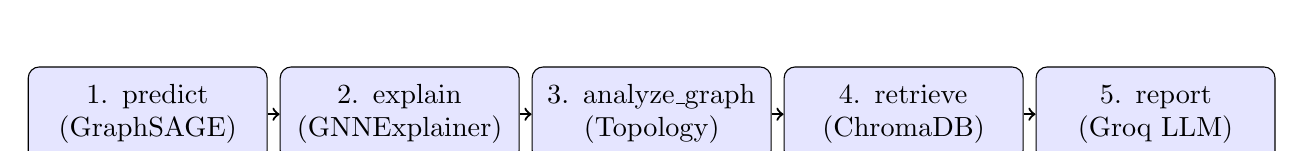
\begin{tikzpicture}[node distance=1.8cm, auto]
  \tikzstyle{block} = [rectangle, draw, fill=blue!10, text width=2.8cm, text centered, rounded corners, minimum height=1.2cm]
  \tikzstyle{line} = [draw, ->, thick]

  \node [block] (pred) {1. predict\\(GraphSAGE)};
  \node [block, right of=pred, node distance=3.2cm] (exp) {2. explain\\(GNNExplainer)};
  \node [block, right of=exp, node distance=3.2cm] (graph) {3. analyze\_graph\\(Topology)};
  \node [block, right of=graph, node distance=3.2cm] (rag) {4. retrieve\\(ChromaDB)};
  \node [block, right of=rag, node distance=3.2cm] (rep) {5. report\\(Groq LLM)};

  \path [line] (pred) -- (exp);
  \path [line] (exp) -- (graph);
  \path [line] (graph) -- (rag);
  \path [line] (rag) -- (rep);
\end{tikzpicture}
\end{center}

\subsection{Execution Steps}
\begin{enumerate}[leftmargin=1.5em]
  \item \textbf{Step 1: \texttt{\_step\_predict}:}
  Calls \texttt{PredictionService.predict\_node(node\_id)}. Computes fraud probabilities, assigns the classification label, and appends the result to \texttt{state["prediction"]}.
  \item \textbf{Step 2: \texttt{\_step\_explain}:}
  Executes \texttt{ExplainabilityService.explain\_node(node\_id)}. Runs GNNExplainer on the extracted 2-hop subgraph to determine the top $K$ features and edge importance weights.
  \item \textbf{Step 3: \texttt{\_step\_graph}:}
  Executes \texttt{GraphAnalysisService.analyze\_node(node\_id)}. Precomputes degree distribution, evaluates 1-hop and 2-hop neighbor illicit ratios, and generates structural flags.
  \item \textbf{Step 4: \texttt{\_step\_rag}:}
  Extracts structural flags and top feature names from state, queries the ChromaDB vector store, and populates \texttt{state["retrieved\_docs"]}.
  \item \textbf{Step 5: \texttt{\_step\_report}:}
  Combines prediction, explanation, topological analysis, and RAG knowledge chunks into a prompt. Dispatches the prompt to the LLM (Groq or Gemini) to generate the final Markdown audit report.
\end{enumerate}

\subsection{Fault Tolerance and Resilience}
If any individual node encounters an exception (e.g., ChromaDB embedding model unavailable or external LLM API rate-limited), the node catches the error, appends the error string to \texttt{state["errors"]}, and gracefully returns partial state. If the LLM call fails, the system executes an automated fallback generator (\texttt{ReportGenerator.\_fallback\_report}), ensuring that the user always receives a complete, structured forensic report.

\chapter{LLM Report Generation and Anti-Hallucination Prompts}

\section{Prompt Engineering Design: \texttt{src/llm/prompts.py}}
A common failure mode in LLM-assisted financial investigations is model hallucination---generating fictional transaction amounts, citing non-existent wallet addresses, or inventing fraudulent narratives unsupported by data.

To prevent hallucinations, \texttt{INVESTIGATION\_PROMPT} employs a strict constraint architecture:
\begin{itemize}[leftmargin=1.5em]
  \item \textbf{Role Definition:} The LLM is initialized as an \textit{"expert cryptocurrency forensic investigator and blockchain AML analyst."}
  \item \textbf{Grounding Rule:} The LLM is explicitly forbidden from inventing transaction data. It is restricted to using only the evidence provided in the prompt sections:
  \begin{itemize}
    \item \texttt{\{prediction\_section\}}: Model probabilities and confidence.
    \item \texttt{\{explanation\_section\}}: Exact feature importances and rank orders.
    \item \texttt{\{graph\_section\}}: Verifiable in/out degrees and neighbor labels.
    \item \texttt{\{rag\_section\}}: Formal typologies retrieved from ChromaDB.
  \end{itemize}
  \item \textbf{Output Structure Enforcement:} The LLM must output exactly five distinct Markdown sections:
  \begin{enumerate}
    \item \textbf{1. RISK ASSESSMENT:} Explicit severity level (LOW, MEDIUM, HIGH) and probability interpretation.
    \item \textbf{2. KEY INDICATORS:} Contrast of local transaction features versus neighborhood aggregate features.
    \item \textbf{3. GRAPH TOPOLOGY \& FLOW OF FUNDS:} Analysis of in/out degree, neighbor illicit ratios, and structural anomaly flags.
    \item \textbf{4. MATCHED TYPOLOGIES:} Correlation of observations with retrieved FATF and AML regulatory patterns.
    \item \textbf{5. RECOMMENDED ACTIONS:} Concrete next steps (e.g., file Suspicious Activity Report / SAR, freeze wallet, add to monitoring watchlist).
  \end{enumerate}
\end{itemize}

\section{Dual-Provider LLM Engine: \texttt{src/llm/report\_generator.py}}
The \texttt{ReportGenerator} class abstracts provider interactions behind a unified interface:
\begin{itemize}[leftmargin=1.5em]
  \item \textbf{Google Gemini Engine:} Uses the official \texttt{google-genai} SDK with \texttt{gemini-2.0-flash} or \texttt{gemini-1.5-flash}. Includes native token budget parameters and thinking config.
  \item \textbf{Groq Cloud Engine:} Uses the OpenAI-compatible \texttt{groq} Python client to target \texttt{openai/gpt-oss-120b} or \texttt{llama-3.3-70b-versatile}. Provides sub-4-second end-to-end report generation.
  \item \textbf{Exponential Backoff Retry Strategy:} If transient HTTP 429 (Rate Limit) or HTTP 503 (Service Unavailable) status codes are received, the client executes an exponential backoff sequence ($1\text{s} \to 2\text{s} \to 4\text{s}$).
\end{itemize}

\chapter{FastAPI Backend and REST Interface}

\section{Application Setup: \texttt{api/main.py}}
The application entry point is built using \textbf{FastAPI}. On startup, the application executes a comprehensive lifecycle initialization sequence via \texttt{@asynccontextmanager}:
\begin{enumerate}[leftmargin=1.5em]
  \item Loads the PyG graph \texttt{elliptic\_graph.pt} and PyTorch model weights \texttt{best\_graphsage.pt}.
  \item Instantiates \texttt{PredictionService}, \texttt{ExplainabilityService}, \texttt{GraphAnalysisService}, and \texttt{InvestigationService}.
  \item Initializes ChromaDB client and verifies collection availability.
  \item Instantiates \texttt{ReportGenerator} and compiles the LangGraph \texttt{InvestigationAgent}.
  \item Binds all instantiated singleton services to \texttt{app.state} for dependency injection into FastAPI routes.
\end{enumerate}

\section{Pydantic Schemas: \texttt{api/schema.py}}
All incoming payloads and outgoing JSON responses are validated through Pydantic models:
\begin{itemize}[leftmargin=1.5em]
  \item \texttt{TransactionRequest}: Dynamically validates arbitrary 166-dimensional numerical feature dictionaries.
  \item \texttt{FraudResponse}: Returns \texttt{fraud\_probability}, \texttt{label} (\texttt{"licit"} or \texttt{"illicit"}), and \texttt{confidence} string.
  \item \texttt{InvestigationRequest}: Configures investigation options (\texttt{include\_shap}, \texttt{explanation\_top\_k}).
  \item \texttt{InvestigationResponse}: Comprehensive JSON model encapsulating \texttt{PredictionDetail}, \texttt{ExplanationDetail}, \texttt{GraphAnalysisDetail}, \texttt{RetrievedDocumentSchema} list, the Markdown \texttt{investigation\_report}, and latency metadata.
\end{itemize}

\section{REST API Endpoints Specification}
\begin{table}[h]
\centering
\small
\begin{tabular}{lllp{6cm}}
\toprule
\textbf{HTTP Method} & \textbf{Path} & \textbf{Input} & \textbf{Description} \\
\midrule
\texttt{GET} & \texttt{/} & None & Serves interactive Cyberpunk frontend dashboard. \\
\texttt{GET} & \texttt{/health} & None & Returns health status of GNN, RAG, and LLM services. \\
\texttt{POST} & \texttt{/predict} & \texttt{TransactionRequest} & Inference from raw 166-feature JSON payload. \\
\texttt{GET} & \texttt{/predict/\{node\_id\}} & Node Index (int) & Fast inference for pre-indexed graph node. \\
\texttt{POST} & \texttt{/investigate/\{node\_id\}} & \texttt{InvestigationRequest} & Full LangGraph agentic investigation pipeline. \\
\texttt{GET} & \texttt{/node/\{node\_id\}} & Node Index (int) & Returns topological degree and neighbor breakdown. \\
\bottomrule
\end{tabular}
\caption{GNN-FraudNet RESTful API Endpoints}
\end{table}

\chapter{Containerization (Docker and Docker Compose)}

To ensure deterministic deployment across heterogeneous host operating systems (macOS ARM64, Linux x86\_64, and Windows), GNN-FraudNet is fully containerized.

\section{The Wheel Strategy and \texttt{Dockerfile}}
Building heavy deep learning frameworks (PyTorch and PyTorch Geometric) inside standard Docker build engines frequently triggers timeout failures and multi-gigabyte virtual network overhead. To eliminate these issues, GNN-FraudNet utilizes a \textbf{Host-Precached Wheel Strategy}:
\begin{enumerate}[leftmargin=1.5em]
  \item Heavy wheels (e.g., \texttt{torch==2.4.0+cpu}) are downloaded locally into a \texttt{docker\_wheels/} directory.
  \item The \texttt{Dockerfile} copies the local wheels directory into the container's \texttt{/tmp/wheels/} and installs with \texttt{--no-index --find-links=/tmp/wheels/}.
  \item Wheels are deleted immediately after installation in the same layer to preserve minimal image size.
  \item Standard application dependencies are installed via \texttt{requirements-docker.txt}.
\end{enumerate}

\begin{lstlisting}[language=bash, caption={Production Dockerfile}]
FROM python:3.11-slim
WORKDIR /app
ENV PIP_DEFAULT_TIMEOUT=300 PIP_RETRIES=5

RUN pip install --no-cache-dir --upgrade pip

# Install PyTorch from cached wheel
COPY docker_wheels/ /tmp/wheels/
RUN pip install --no-cache-dir --no-index --find-links=/tmp/wheels/ torch==2.4.0 && \
    rm -rf /tmp/wheels/

# Install remaining inference dependencies
COPY requirements-docker.txt .
RUN pip install --no-cache-dir -r requirements-docker.txt

# Copy application assets and pre-trained artifacts
COPY src/ ./src/
COPY api/ ./api/
COPY results/best_graphsage.pt ./results/best_graphsage.pt
COPY data/processed/elliptic_graph.pt ./data/processed/elliptic_graph.pt

RUN mkdir -p /app/knowledge_base
EXPOSE 8000
CMD ["uvicorn", "api.main:app", "--host", "0.0.0.0", "--port", "8000"]
\end{lstlisting}

\section{Docker Compose Configuration: \texttt{docker-compose.yml}}
The container lifecycle, port mappings, volume mounts, and automated health checks are declared in \texttt{docker-compose.yml}:
\begin{lstlisting}[language=bash, caption={docker-compose.yml}]
version: "3.8"
services:
  app:
    build:
      context: .
      dockerfile: Dockerfile
    ports:
      - "127.0.0.1:8000:8000"
    env_file:
      - .env
    environment:
      - MODEL_PATH=results/best_graphsage.pt
      - DATA_PATH=data/processed/elliptic_graph.pt
      - CHROMA_DB_PATH=knowledge_base/chroma_db
      - LOG_LEVEL=INFO
    volumes:
      - ./knowledge_base:/app/knowledge_base
    restart: unless-stopped
    healthcheck:
      test: ["CMD", "python", "-c", "import urllib.request; urllib.request.urlopen('http://localhost:8000/health')"]
      interval: 30s
      timeout: 10s
      retries: 3
      start_period: 60s
\end{lstlisting}
Notice that the container port is bound exclusively to \texttt{127.0.0.1:8000}, preventing direct external access and enforcing traffic routing through Nginx.

\chapter{AWS Production Deployment and Troubleshooting}

\section{AWS Cloud Environment Specifications}
The production deployment was provisioned on Amazon Web Services (AWS) EC2:
\begin{itemize}[leftmargin=1.5em]
  \item \textbf{Instance Type:} \texttt{m7i-flex.large} (Latest-generation Intel Xeon 8488C processors).
  \item \textbf{Compute \& Memory:} 2 vCPUs, 8 GiB RAM (essential for loading the 141 MB PyG graph and holding embedding models in memory).
  \item \textbf{Storage:} 30 GiB General Purpose SSD (gp3) EBS volume.
  \item \textbf{Operating System:} Ubuntu Server 24.04 LTS (x86\_64).
  \item \textbf{Networking \& Reverse Proxy:} Nginx reverse proxy fronting Docker.
\end{itemize}

\section{Reverse Proxy and Network Security Design}
To achieve network isolation, the network architecture decouples the public internet from the application container:
\begin{lstlisting}[caption=Production Network Path]
Browser / Client (Port 80)
           |
AWS Security Group (Allow Port 80 from 0.0.0.0/0; Port 22 from Client IP/32)
           |
Nginx Reverse Proxy (/etc/nginx/sites-available/gnn-fraudnet)
           |  (proxy_pass http://127.0.0.1:8000)
Internal Loopback (127.0.0.1:8000)
           |
Docker Container (FastAPI Microservice)
\end{lstlisting}

\subsection{Nginx Configuration}
The reverse proxy configuration deployed under \texttt{/etc/nginx/sites-available/gnn-fraudnet}:
\begin{lstlisting}
server {
    listen 80;
    server_name <EC2_PUBLIC_IP>;

    location / {
        proxy_pass http://127.0.0.1:8000;
        proxy_set_header Host $host;
        proxy_set_header X-Real-IP $remote_addr;
        proxy_set_header X-Forwarded-For $proxy_add_x_forwarded_for;
        proxy_set_header X-Forwarded-Proto $scheme;
    }
}
\end{lstlisting}


\section{Deployment Runbook and Operational Checks}

A clean deployment follows the sequence below:

\begin{enumerate}[leftmargin=1.5em]
  \item Provision the EC2 instance and restrict the security group to the required inbound ports.
  \item Install Docker/Docker Compose and verify that the daemon is healthy.
  \item Transfer large graph/model artifacts separately from the source repository.
  \item Verify SHA-256 checksums for transferred binary artifacts.
  \item Build the application image using the destination architecture and CPU-only dependency set.
  \item Start the service with Docker Compose and inspect application logs.
  \item Verify the internal FastAPI health endpoint.
  \item Configure and validate Nginx with \texttt{nginx -t}.
  \item Verify the public endpoint through the Nginx path.
  \item Execute a representative prediction and a complete investigation request.
\end{enumerate}

Useful operational commands include:

\begin{lstlisting}[language=bash]
docker compose ps
docker compose logs --tail=100 app
docker compose restart app
curl http://127.0.0.1:8000/health
curl http://<EC2_PUBLIC_IP>/health
sudo nginx -t
sudo systemctl status nginx
\end{lstlisting}

These checks intentionally progress from the inside out: container health first, local API second, reverse proxy third, and public access last. This ordering significantly reduces debugging ambiguity.

\section{Security, Reliability, and Production Considerations}

The deployment is a \textbf{production-oriented prototype}, not a fully certified financial-compliance platform. The current security posture includes network-level port restrictions, Nginx reverse proxying, separation of secrets from source code, and non-public exposure of the FastAPI application port. For a larger deployment, the following controls would be appropriate:

\begin{itemize}[leftmargin=1.5em]
  \item HTTPS with managed certificates and automatic renewal.
  \item Authentication and authorization for investigation endpoints.
  \item Rate limiting and request-size limits at the reverse proxy.
  \item Structured application logs with request identifiers.
  \item Centralized monitoring for CPU, RAM, latency, error rates, and LLM-provider failures.
  \item Secrets management through AWS Secrets Manager or an equivalent service instead of long-lived environment-file secrets.
  \item Automated image scanning and dependency vulnerability checks.
  \item Immutable model/data versioning so an investigation can be reproduced from the exact artifact versions used at inference time.
  \item Audit logs that record the model version, prediction, explanation configuration, retrieved documents, and LLM provider used for every investigation.
\end{itemize}

These controls are particularly important for fraud-analysis systems because a generated report should be traceable to the evidence and model state that produced it.

\section{Exhaustive Engineering Challenges and Resolutions}
Deploying deep learning systems to production clouds exposes severe edge cases across hardware architectures, memory management, and package boundaries. Below is the complete record of engineering challenges diagnosed and resolved:

\subsection{Problem 1: SSH Pipe Breakage on Unstable Networks}
\begin{itemize}[leftmargin=1.5em]
  \item \textbf{Symptom:} AWS Instance Connect dropped unexpectedly, and direct SSH sessions experienced frequent \texttt{client\_loop: send disconnect: Broken pipe} terminations.
  \item \textbf{Diagnosis:} Upstream cellular NAT firewalls silently dropped idle TCP connections.
  \item \textbf{Resolution:} Configured client-side SSH keepalive intervals:
  \begin{lstlisting}[language=bash]
  ssh -o ServerAliveInterval=30 -o ServerAliveCountMax=3 -i key.pem ubuntu@<IP>
  \end{lstlisting}
\end{itemize}

\subsection{Problem 2: Missing Graph Artifact in Git Repository}
\begin{itemize}[leftmargin=1.5em]
  \item \textbf{Symptom:} Initial container builds failed with \texttt{FileNotFoundError: data/processed/elliptic\_graph.pt}.
  \item \textbf{Diagnosis:} The processed graph file ($\approx 141$ MB) exceeded GitHub's 100 MB file limit and was appropriately ignored by \texttt{.gitignore}.
  \item \textbf{Resolution:} Transferred the artifact directly via secure SCP and validated cryptographic integrity using SHA-256 checksums:
  \begin{lstlisting}[language=bash]
  # Checksums validated identical across host and EC2:
  e05d1ca6a69e324f7ce5ebace75041df7746fa6b8115e5719fcf0a8411dbcdd3  elliptic_graph.pt
  fc84d65da12a9428518e3be2722cc2e1ef14649a4f26b33d7fe3d259e0fdafce  best_graphsage.pt
  \end{lstlisting}
\end{itemize}

\subsection{Problem 3: Architecture Mismatch on Pre-downloaded Wheels}
\begin{itemize}[leftmargin=1.5em]
  \item \textbf{Symptom:} Docker install failed with \texttt{torch-2.4.0-cp311-...-aarch64.whl is not a supported wheel on this platform}.
  \item \textbf{Diagnosis:} The host development machine was an Apple Silicon Mac (ARM64), whereas the EC2 instance was an Intel Xeon (x86\_64).
  \item \textbf{Resolution:} Explicitly targeted the destination architecture using pip download flags:
  \begin{lstlisting}[language=bash]
  docker run --rm -v "$PWD/docker_wheels:/wheels" python:3.11-slim \
    pip download torch==2.4.0 --index-url https://download.pytorch.org/whl/cpu \
    --python-version 311 --platform linux_x86_64 --only-binary=:all: --no-deps -d /wheels
  \end{lstlisting}
\end{itemize}

\subsection{Problem 4: Unwanted CUDA Dependencies in Local Wheel Cache}
\begin{itemize}[leftmargin=1.5em]
  \item \textbf{Symptom:} Docker build attempted to download NVIDIA CUDA runtime dependencies ($> 2.5$ GB) and failed due to \texttt{--no-index}.
  \item \textbf{Diagnosis:} Standard PyPI PyTorch packages default to CUDA-enabled binaries.
  \item \textbf{Resolution:} Downloaded the dedicated CPU-only build (\texttt{torch==2.4.0+cpu}), which is only 187 MB and requires no GPU drivers.
\end{itemize}

\subsection{Problem 5: Dependency Incompatibility Between Transformers and PyTorch 2.4.0}
\begin{itemize}[leftmargin=1.5em]
  \item \textbf{Symptom:} Server crashed during startup with:
  \begin{lstlisting}
  [transformers] Disabling PyTorch because PyTorch >= 2.5 is required but found 2.4.0+cpu
  NameError: name 'nn' is not defined
  \end{lstlisting}
  \item \textbf{Diagnosis:} The latest unpinned \texttt{transformers} library dropped backward compatibility for PyTorch 2.4.0, deactivating internal neural network modules.
  \item \textbf{Resolution:} Explicitly pinned compatible releases in \texttt{requirements-docker.txt}:
  \begin{lstlisting}
  sentence-transformers==3.3.1
  transformers==4.46.3
  \end{lstlisting}
\end{itemize}

\subsection{Problem 6: Gemini Free-Tier Quota Exhaustion}
\begin{itemize}[leftmargin=1.5em]
  \item \textbf{Symptom:} Investigation requests began failing after multiple live demos with:
  \begin{lstlisting}
  HTTP 429 Too Many Requests | RESOURCE_EXHAUSTED | generate_content_free_tier_requests
  \end{lstlisting}
  \item \textbf{Diagnosis:} Google Gemini free-tier imposes restrictive minute and daily request quotas. Retries across 3 attempts added $\approx 7$ seconds of useless latency.
  \item \textbf{Resolution:} Refactored \texttt{ReportGenerator} to support dynamic multi-provider configuration via \texttt{.env}. Migrated the primary production engine to \textbf{Groq Cloud} (\texttt{openai/gpt-oss-120b}), reducing investigation latency from $\mathbf{8.5s \to 3.73s}$.
\end{itemize}

\chapter{End-to-End Verification and Forensic Case Study}

\section{Production Health Status}
Following container startup and Nginx binding, querying \texttt{http://<EC2\_PUBLIC\_IP>/health} verified that all subsystems initialized correctly:
\begin{lstlisting}[language=bash]
{
  "status": "ok",
  "model": "GraphSAGE",
  "rag_available": true,
  "llm_available": true,
  "investigation_available": true
}
\end{lstlisting}

\section{Case Study: Forensic Investigation of Node 78642}
A full end-to-end investigation was executed against transaction node \textbf{78642} on the public AWS deployment:
\begin{lstlisting}[language=bash]
curl -X POST http://<EC2_PUBLIC_IP>/investigate/78642 \
  -H "Content-Type: application/json" \
  -d '{"include_shap": false, "explanation_top_k": 10}'
\end{lstlisting}
Total end-to-end execution time: \textbf{3.739 seconds}.

\subsection{Quantitative Predictions and Graph Topology}
\begin{itemize}[leftmargin=1.5em]
  \item \textbf{Model Prediction:}
  \begin{itemize}
    \item Fraud Probability: $0.1628$ ($16.28\%$)
    \item Licit Probability: $0.8372$ ($83.72\%$)
    \item Label: \texttt{"licit"}
    \item Confidence: \texttt{"high"}
  \end{itemize}
  \item \textbf{Graph Topology Metrics:}
  \begin{itemize}
    \item In-degree: 1, Out-degree: 1, Total Degree: 2
    \item 1-Hop Neighbors: 1 unknown, 0 licit, 0 illicit
    \item 2-Hop Neighbors: 2 unknown, 0 licit, 0 illicit
    \item Structural Flag: \texttt{"mostly\_unknown\_neighbors"}
  \end{itemize}
\end{itemize}

\subsection{Top-10 GNNExplainer Attributed Features}
\begin{longtable}{cccc}
\toprule
\textbf{Rank} & \textbf{Feature Identifier} & \textbf{Importance Score} & \textbf{Category} \\
\midrule
1 & \texttt{feature\_149} & 0.8735 & Neighborhood Aggregate \\
2 & \texttt{feature\_161} & 0.8727 & Neighborhood Aggregate \\
3 & \texttt{feature\_7}   & 0.8507 & Local Transaction Fee/Volume \\
4 & \texttt{feature\_5}   & 0.8410 & Local Transaction Feature \\
5 & \texttt{feature\_64}  & 0.8193 & Local Transaction Feature \\
6 & \texttt{feature\_116} & 0.7794 & Neighborhood Aggregate \\
7 & \texttt{feature\_158} & 0.6820 & Neighborhood Aggregate \\
8 & \texttt{feature\_22}  & 0.6509 & Local Transaction Feature \\
9 & \texttt{feature\_148} & 0.6390 & Neighborhood Aggregate \\
10 & \texttt{feature\_54} & 0.6360 & Local Transaction Feature \\
\bottomrule
\end{longtable}

\subsection{Generated Natural-Language Forensic Report}
The Groq LLM synthesized the following intelligence report:
\begin{tcolorbox}[colback=boxbg,colframe=darkblue,title=\textbf{Generated Forensic Investigation Audit Report}]
\small
\textbf{1. RISK ASSESSMENT}\\
\textbf{Severity Level:} LOW\\
\textbf{Confidence Score:} HIGH (83.72\% Licit Probability)\\
Node 78642 exhibits an estimated fraud probability of 16.28\%, categorizing it well below the illicit threshold of 0.70. The model explicitly designates this entity as licit with high confidence.

\vspace{0.3cm}
\textbf{2. KEY INDICATORS}\\
The GNNExplainer analysis demonstrates that neighborhood aggregate metrics exerted the strongest influence on this prediction. Specifically, \texttt{feature\_149} (importance: 0.8735) and \texttt{feature\_161} (importance: 0.8727) dominate the attribution space, indicating that the statistical variance of the input transactions aligns with standard commercial wallet patterns rather than money-laundering structuring. Local features \texttt{feature\_7} and \texttt{feature\_5} confirm standard fee ratios.

\vspace{0.3cm}
\textbf{3. GRAPH TOPOLOGY \& FLOW OF FUNDS}\\
Topological analysis reveals that Node 78642 is a standard pass-through transaction with an in-degree of 1 and an out-degree of 1. It possesses zero 1-hop and zero 2-hop illicit associations. The system flagged \texttt{mostly\_unknown\_neighbors} due to adjacent unannotated wallets; however, in the absence of fan-in or peeling structures, this reflects standard private transfers rather than an intentional tumbling pattern.

\vspace{0.3cm}
\textbf{4. MATCHED TYPOLOGIES}\\
Cross-referencing the retrieved knowledge base reveals that this transaction does not match darknet marketplace payout structures or high-velocity peeling chains. The single-input, single-output structure with normal transaction fees is consistent with benign peer-to-peer transfers or standard cold-storage consolidation.

\vspace{0.3cm}
\textbf{5. RECOMMENDED ACTIONS}\\
1. Clear the automated flag on Node 78642; no suspicious activity report (SAR) is required at this time.\\
2. Maintain standard passive monitoring on adjacent unannotated successor wallets.\\
3. Log the GNNExplainer feature attribution vector to the compliance audit trail.
\end{tcolorbox}


\chapter{Engineering Lessons Learned}

\section{What Changed Between the Notebook and Production}

The most important lesson from the project is that model development and system engineering impose different failure modes. The GNN itself was only one part of the final system. The production path required solving:

\begin{itemize}[leftmargin=1.5em]
  \item \textbf{Artifact management:} the processed graph and model weights were too large for ordinary source-control handling.
  \item \textbf{Architecture portability:} development occurred on Apple Silicon (ARM64), while the target EC2 machine used x86\_64 Intel CPUs.
  \item \textbf{Dependency determinism:} unpinned ML packages introduced incompatibilities that were not visible during initial experimentation.
  \item \textbf{Latency engineering:} explainability methods that are acceptable offline can become unacceptable inside a synchronous API request.
  \item \textbf{External service reliability:} LLM quota exhaustion demonstrated why provider abstraction and graceful failure paths matter.
  \item \textbf{Observability:} health endpoints and container logs were essential for distinguishing application failures from infrastructure failures.
\end{itemize}

\section{Why the Architecture Is Modular}

The modular design provides a practical upgrade path. A future version can replace GraphSAGE with a temporal GNN without rewriting the RAG subsystem; replace ChromaDB without changing graph inference; add another LLM provider without modifying the graph-analysis service; or move from a single EC2 instance to a managed container platform without changing the core investigation state machine.

This is the primary architectural value of the project: \textbf{the ML model is treated as one component in a larger evidence-processing system rather than as the entire application}.

\chapter{Conclusion, Codebase Directory, and Future Work}

\section{Summary of Engineering Achievements}
GNN-FraudNet demonstrates the successful transformation of an advanced Graph Neural Network research model into an production-oriented, explainable, and operational cloud microservice. Key accomplishments include:
\begin{itemize}[leftmargin=1.5em]
  \item Achieved a benchmark illicit PR-AUC of 0.917 using GraphSAGE on the 203,769-node Elliptic dataset.
  \item Solved the $k$-hop subgraph extraction challenge to drop GNNExplainer latency from 45 seconds to under 0.5 seconds.
  \item Built a RAG knowledge base backed by ChromaDB and sentence-transformers to ground LLM reasoning in verified AML typologies.
  \item Orchestrated stateful multi-step reasoning using LangGraph to deliver complete fraud reports in 3.73 seconds.
  \item Containerized the entire deep learning runtime and deployed securely to AWS EC2 behind a Nginx reverse proxy.
\end{itemize}

\section{Complete Project Directory Tree}
Below is the exhaustive directory and file layout of the \texttt{GNN-FraudNet} repository:
\begin{lstlisting}
GNN-FraudNet/
+-- .env.example                     # Environment template (API keys, ports, paths)
+-- .gitignore                       # Ignored artifacts (data/raw, .venv, .env)
+-- .dockerignore                    # Excluded from container build
+-- Dockerfile                       # Multi-stage CPU-optimized container definition
+-- docker-compose.yml               # Service orchestration and volume mounts
+-- requirements.txt                 # Host development dependencies
+-- requirements-docker.txt          # Pinned container inference dependencies
+-- README.md                        # Master project documentation
+-- project_overview.md              # Conceptual guide and architecture diagrams
+-- aws.json                         # Sample raw production response from AWS
+-- check_transaction.py             # CLI utility to query single nodes
+-- test_predict.py                  # Standalone API test script
+-- api/
|   +-- main.py                      # FastAPI application, lifecycle, and endpoints
|   +-- schema.py                    # Pydantic data validation schemas
|   `-- static/
|       `-- index.html               # Cyberpunk frontend single-page dashboard
+-- data/
|   +-- raw/                         # Raw Elliptic CSV files (txs_features, classes, edgelist)
|   `-- processed/
|       `-- elliptic_graph.pt        # Serialized PyTorch Geometric Data graph object
+-- docker_wheels/                   # Pre-downloaded x86_64 CPU-only PyTorch wheels
+-- notebooks/
|   +-- 01_eda.ipynb                 # Exploratory data analysis on Elliptic dataset
|   +-- 02_graph_construction.ipynb  # PyG Data construction and mask generation
|   +-- 03_baseline_models.ipynb     # LogReg, Random Forest, and XGBoost training
|   `-- 04_gnn_training.ipynb        # GraphSAGE / GAT training, loss curves, and XAI
+-- results/
|   +-- best_graphsage.pt            # Serialized optimal GraphSAGE weights
|   +-- best_gat.pt                  # Serialized GAT weights
|   `-- metrics_comparison.csv       # Benchmark tabular metrics across all models
+-- src/
|   +-- __init__.py
|   +-- config.py                    # Centralized settings and environment loader
|   +-- data_loader.py               # Ingestion of raw CSVs into memory
|   +-- graph_builder.py             # Normalization, temporal masks, train/val/test splits
|   +-- train.py                     # GNN training loop, class-weighting, early stopping
|   +-- evaluate.py                  # Calculation of PR-AUC, F1, and confusion matrices
|   +-- explain.py                   # Offline batch GNNExplainer and SHAP scripts
|   +-- models/
|   |   +-- __init__.py
|   |   +-- graphsage.py             # GraphSAGE PyTorch Geometric implementation
|   |   +-- gat.py                   # Graph Attention Network implementation
|   |   `-- baseline.py              # Scikit-learn and XGBoost baseline wrappers
|   +-- services/
|   |   +-- __init__.py
|   |   +-- prediction.py            # Real-time GNN inference service
|   |   +-- explainability.py        # Subgraph-accelerated GNNExplainer and SHAP
|   |   +-- graph_analysis.py        # Topological degree and neighbor ratio analyzer
|   |   `-- investigation.py         # Multi-service context aggregation layer
|   +-- rag/
|   |   +-- __init__.py
|   |   +-- knowledge_base.py        # ChromaDB vector store initialization and chunking
|   |   +-- retriever.py             # Dense semantic similarity search
|   |   `-- documents/               # Markdown domain intelligence briefs
|   |       `-- fraud_typologies.md  # Detailed AML red flags, peeling chains, mixers
|   +-- llm/
|   |   +-- __init__.py
|   |   +-- prompts.py               # Anti-hallucination structured prompt templates
|   |   `-- report_generator.py      # Multi-provider client (Groq / Gemini) with fallback
|   `-- agents/
|       +-- __init__.py
|       `-- investigation_agent.py   # LangGraph StateGraph agentic workflow
`-- tests/
    +-- test_prediction.py           # Unit tests for GNN inference
    +-- test_explainability.py       # Unit tests for subgraph extraction and XAI
    `-- test_api.py                  # Integration tests for FastAPI endpoints
\end{lstlisting}


\section{Current Limitations and Responsible Use}

Several limitations should be made explicit.

\begin{enumerate}[leftmargin=1.5em]
  \item \textbf{Benchmark dependence:} the reported metrics are obtained on the Elliptic benchmark and should not be interpreted as universal performance on contemporary cryptocurrency activity.
  \item \textbf{Label sparsity:} a large fraction of the graph is unlabeled. ``Unknown'' is not equivalent to ``licit'' and should remain a separate analytical state.
  \item \textbf{Class imbalance:} the illicit class is much smaller than the licit class, making accuracy alone an insufficient measure of detection quality.
  \item \textbf{Temporal drift:} fraud strategies evolve. A model trained on historical transactions can degrade when deployed against new behavioral patterns.
  \item \textbf{Explainability is not causality:} GNNExplainer and SHAP identify features or graph components associated with a prediction; they do not prove that those features caused the illicit behavior.
  \item \textbf{LLM output is advisory:} generated prose should summarize and contextualize structured evidence, not replace analyst judgment or legal/compliance review.
  \item \textbf{External-provider dependence:} LLM availability, rate limits, latency, and pricing can change. Provider abstraction and fallback behavior are therefore operational requirements rather than optional conveniences.
\end{enumerate}

For these reasons, GNN-FraudNet should be treated as a decision-support and investigation system. A high-risk prediction is a signal for further analysis, not by itself proof of criminal activity.

\section{Future Research and System Enhancements}
\begin{enumerate}[leftmargin=1.5em]
  \item \textbf{Dynamic Graph Updating:} Currently, inference operates over the pre-indexed Elliptic graph. Future iterations will incorporate dynamic graph stream insertion (e.g., utilizing PyG's \texttt{NeighborLoader} or temporal GNNs such as TGN) to process streaming mempool transactions in real time.
  \item \textbf{Hardware Acceleration:} For high-throughput banking clusters ($> 10,000$ tx/sec), migrating the inference service to AWS Inferentia or NVIDIA TensorRT can improve throughput and latency when benchmarked and tuned for the target workload.
  \item \textbf{Automated SAR Submission:} Expanding the LangGraph agent to generate analyst-reviewable SAR-ready structured outputs, with any final regulatory submission remaining under authorized human/compliance control.
  \item \textbf{TLS / HTTPS and Custom Domain:} Provisioning an automated Let's Encrypt SSL/TLS certificate via Certbot inside Nginx to enable encrypted HTTPS communication.
\end{enumerate}

\end{document}
